\documentclass[]{article}
\usepackage[spanish]{babel}
\usepackage{graphicx}
\usepackage{float} 
\usepackage{standalone}
\usepackage{adjustbox}
\usepackage{longtable} 
\usepackage{booktabs} 
\usepackage{rotating} 
\usepackage{float}
\usepackage{amsmath}
\usepackage{enumitem}
\setlength{\parindent}{0pt} 
\graphicspath{{C:/Users/USER/Documents/econometria/tarea1/plot/}}
\usepackage[letterpaper]{geometry}


%opening
\title{Problem Set 1}
\author{Tannya Mainato \and Alan Del Rosario \and Mariuxi Gualán}
\date{2024}

\begin{document}
\maketitle
\section*{Pregunta 1}

Gráfica de cada línea:

\begin{enumerate}[label=\alph*)]
	\item $\sqrt{3+2x}$ 
\end{enumerate}

\begin{enumerate}[label=\alph*)]
	\item $y=-2-\frac{1}{2}x$
\end{enumerate}

\section*{Pregunta 2}
Encuentra la ecuación de la línea recta que pasa por los puntos:

\begin{enumerate} [label=\alph*)]
	\item $(0,3) y (4,0)$
\end{enumerate}



\begin{enumerate} [label=\alph*)]
	\item $(2,-3) y (6,5)$
\end{enumerate}
 
\section*{Pregunta 3}
Dada la ecuación: 

$$y=-1+2x_1-\frac{1}{2}x_2+3x_3$$

Encuentra el valor de $y$ cuando $x_1=3$, $x_2=4$ y $x_3=5$.

\section*{Pregunta 4}
Calcula las siguientes sumatorias:

\begin{enumerate}[label=(\alph*)]
	\item $\sum_{i=1}^{5}i$
	\item $\sum_{i=1}^{6}2i$
	\item $\sum_{i=1}^{4}(3i-1)$	
	\item $\sum_{i=1}^{3}(2i+1)^2$	
\end{enumerate}

\section*{Pregunta 5}
¿Cuál es la sumatoria de $\sum_{i=1}^{5}1$?

\begin{figure}[H]
	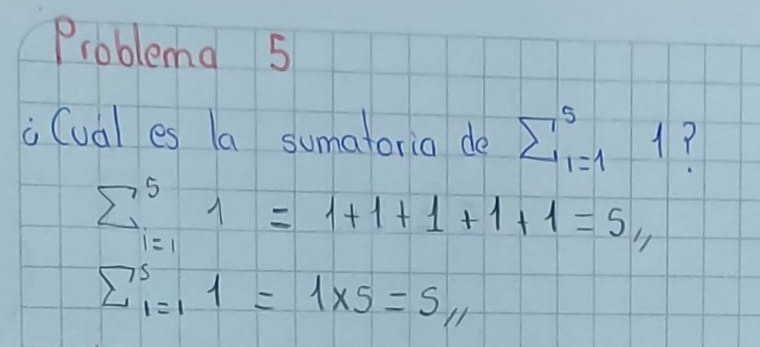
\includegraphics{/Pregunta_5/5_a.jpg}
\end{figure}

\section*{Pregunta 6}
Calcula las siguientes derivadas. No es necesario simplificar.

\begin{enumerate}[label=(\alph*)]
	\item Encuentra $\frac{dy}{dx}$ de $y=3x^2$
	\item Encuentra $\frac{dy}{dx}$ de $y=4x^{-3}+2$
	\begin{figure}[H]
		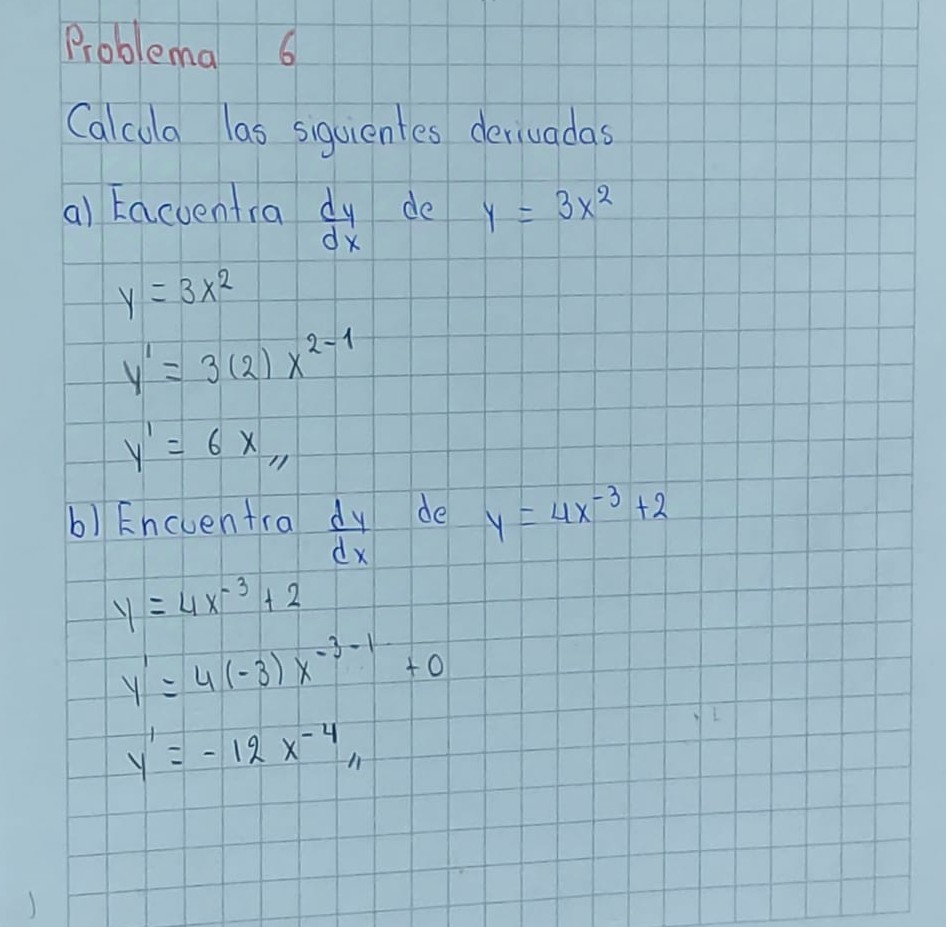
\includegraphics[width=1\linewidth]{/Pregunta_6/6_a_b.jpg}
	\end{figure}
	\item Encuentra $\frac{df(x)}{dx}$ de $f(x)=2x^{-1/2} - 6x$
	\item Encuentra $\frac{df(x)}{dx}$ de $f(x)=3x^2-4x+1$
	\begin{figure}[H]
	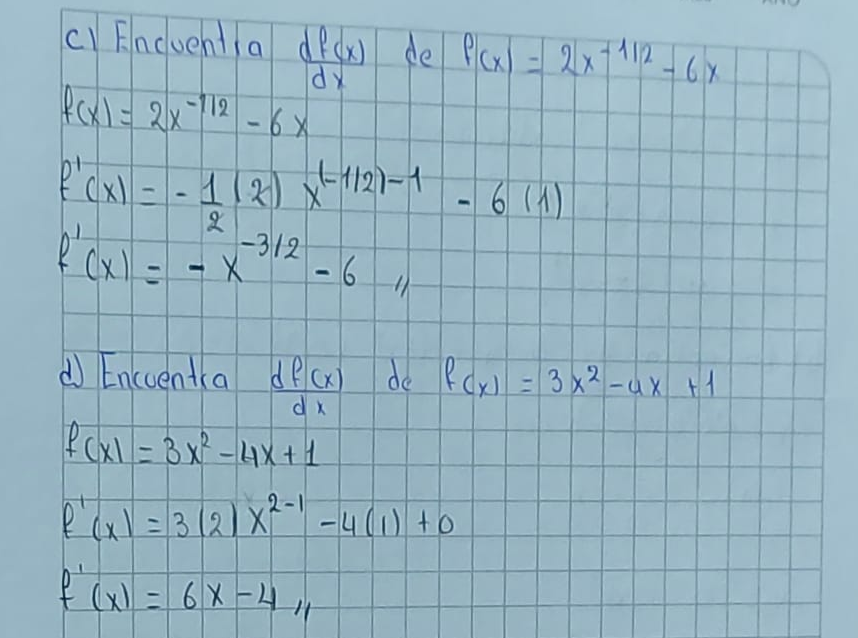
\includegraphics[width=1\linewidth]{/Pregunta_6/6_c_d.png}
	\end{figure}
\end{enumerate}

\section*{Pregunta 7}
Calcula las siguientes derivadas utilizando la regla de la cadena. No es necesario simplificar.

\begin{enumerate}[label=\alph*]
	\item Encuentra $\frac{dy}{dx}$ de $y=(2x+3)^5$
	\begin{figure}[H]
		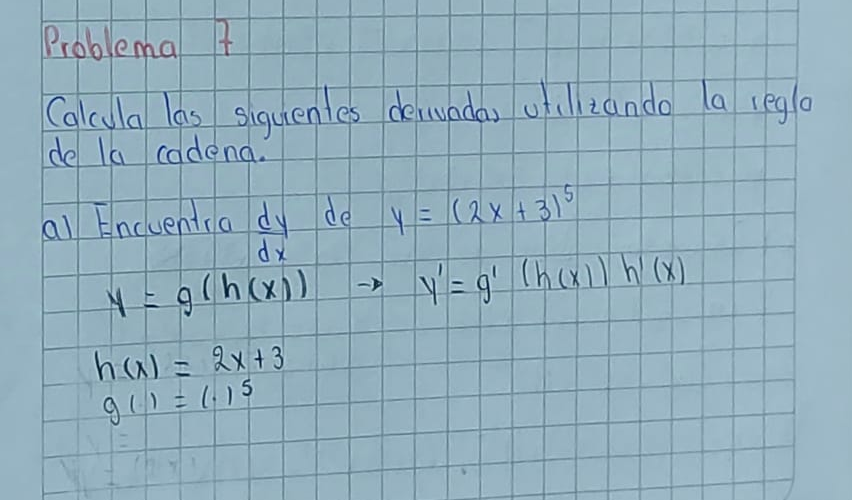
\includegraphics[width=1\linewidth]{/Pregunta_7/7_a.png}
	\end{figure}
	\item Encuentra $\frac{dy}{dy}$ de $y=(3x^2+2x)^3$
	\item Encuentra $\frac{df(x)}{dx}$ de $f(x)=(2x^3-3x^2+1)^2$
	\begin{figure}[H]
	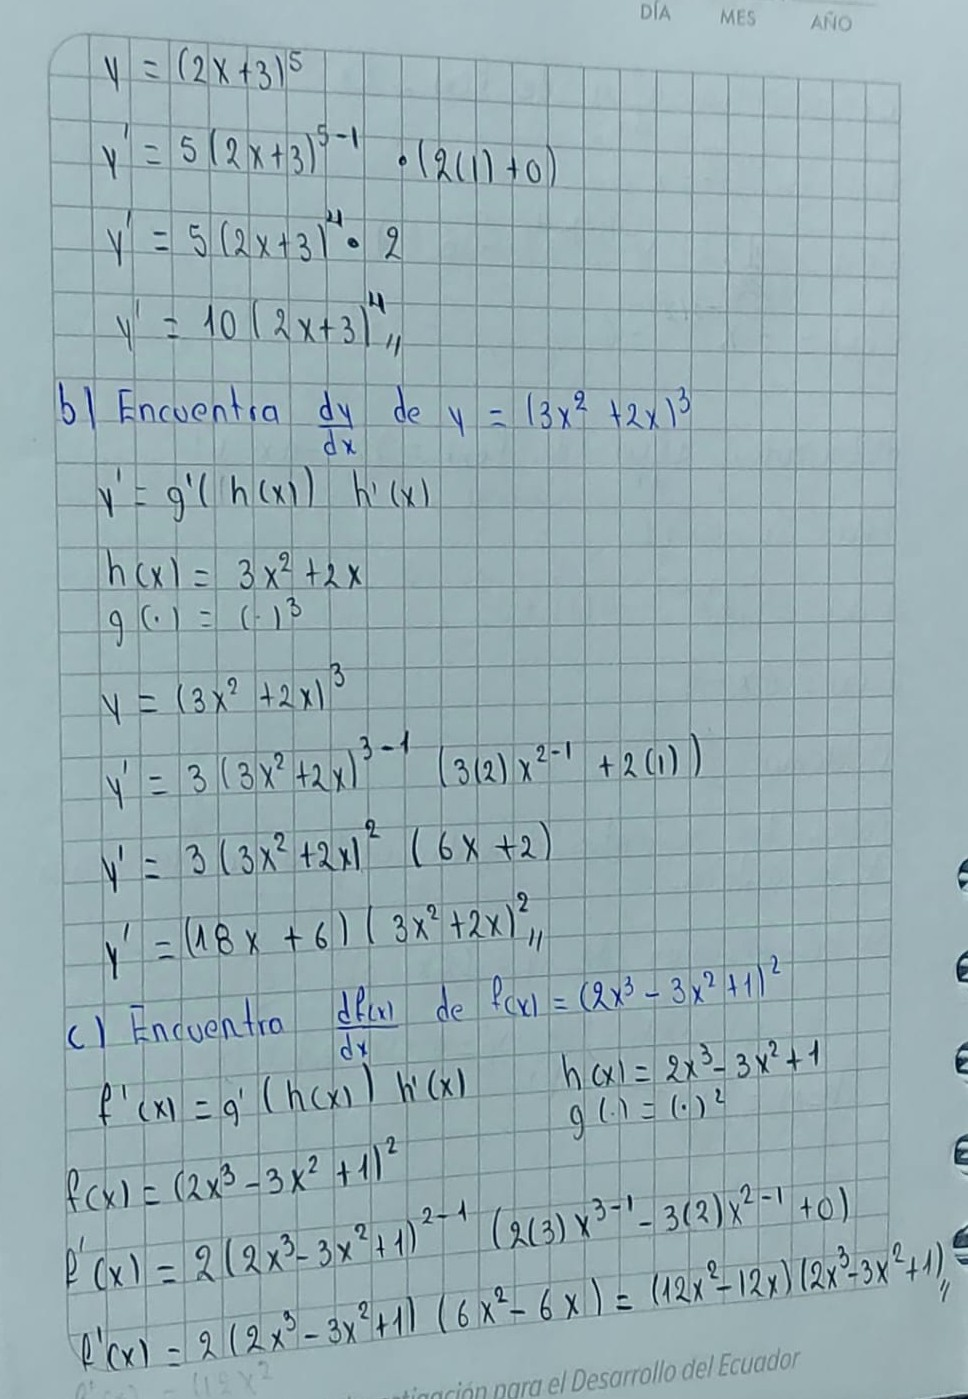
\includegraphics[width=1\linewidth]{/Pregunta_7/7_b_c.png}
	\end{figure}
	\item Encuentra $\frac{df(x)}{dx}$ de $f(x)=(2x^2+5)^{\frac{1}{2}}$ 
	\begin{figure}[H]
		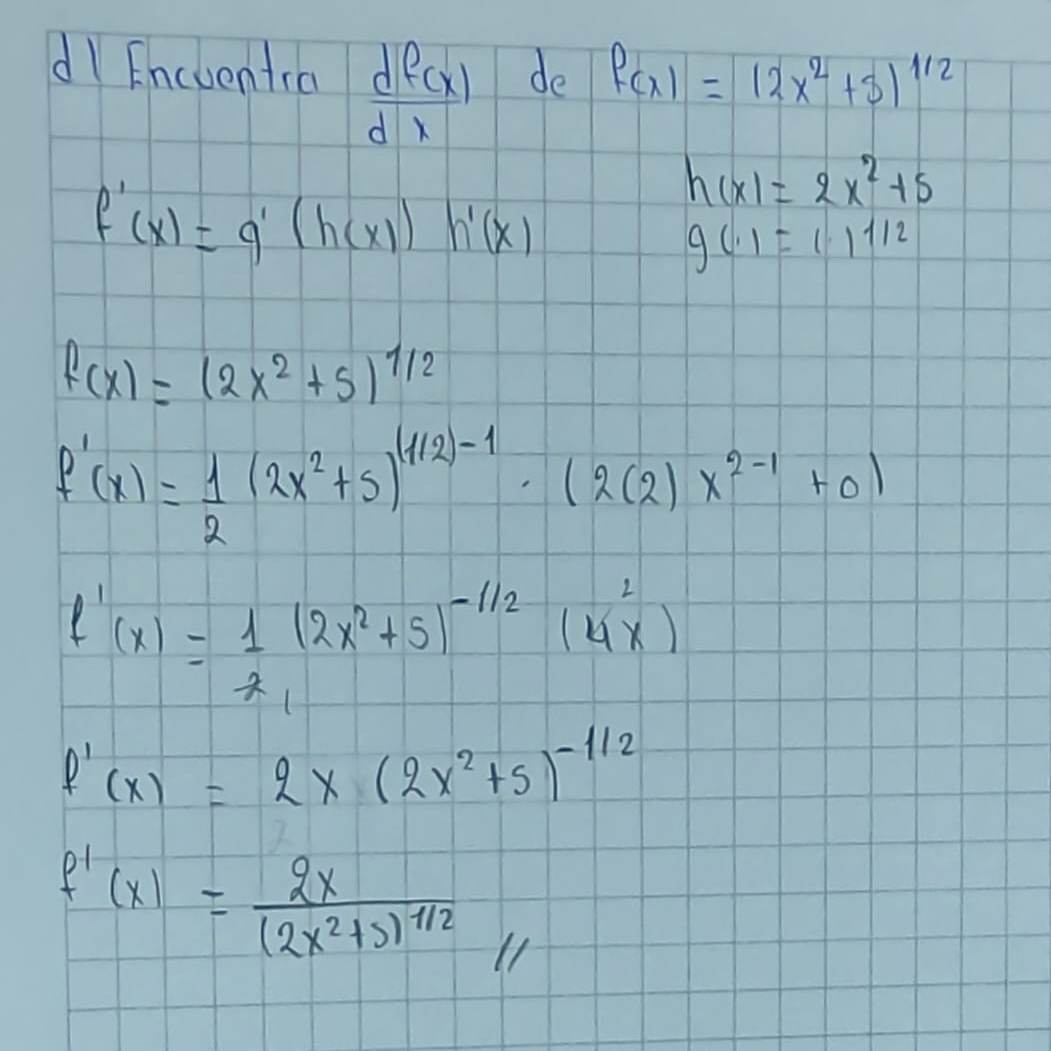
\includegraphics[width=1\linewidth]{/Pregunta_7/7_d.png}
	\end{figure}
\end{enumerate}

\section*{Pregunta 8}
Calcula llas siguientes derivadas parciales. No es necesario simplificar.

\begin{enumerate}[label=(\alph*)]
	\item Encuentra $\frac{\partial z}{\partial x}$ y $\frac{\partial z}{\partial y}$ de $z=3^2+2y^3$
	\begin{figure}[H]
		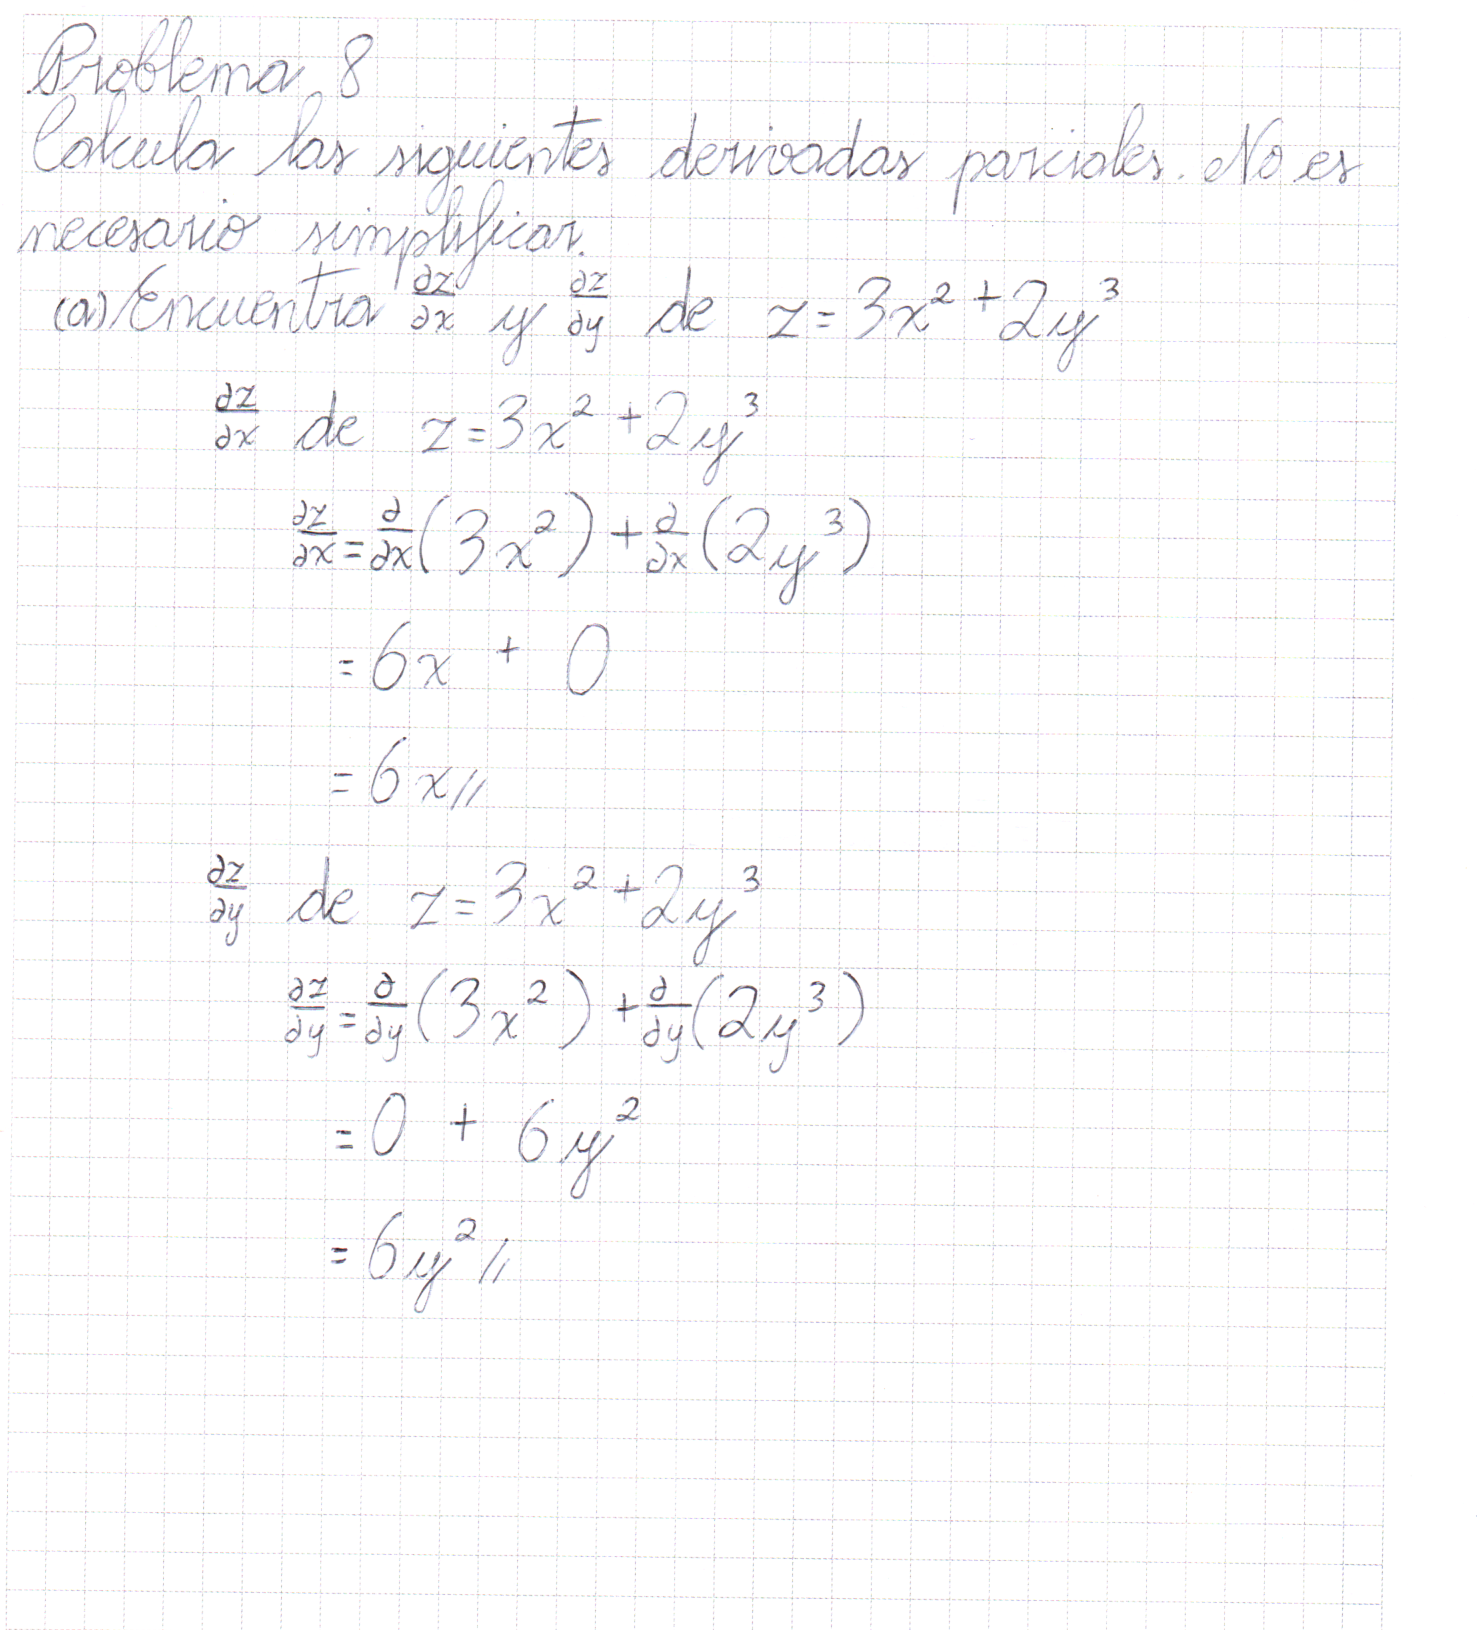
\includegraphics[width=1\linewidth]{/pregunta_8/8_a.png}
	\end{figure}
	\item Encuentra $\frac{\partial z}{\partial x}$ y $\frac{\partial z}{\partial y}$ de $z=(3x-y+1)^\frac{1}{2}$.
	\begin{figure}[H]
		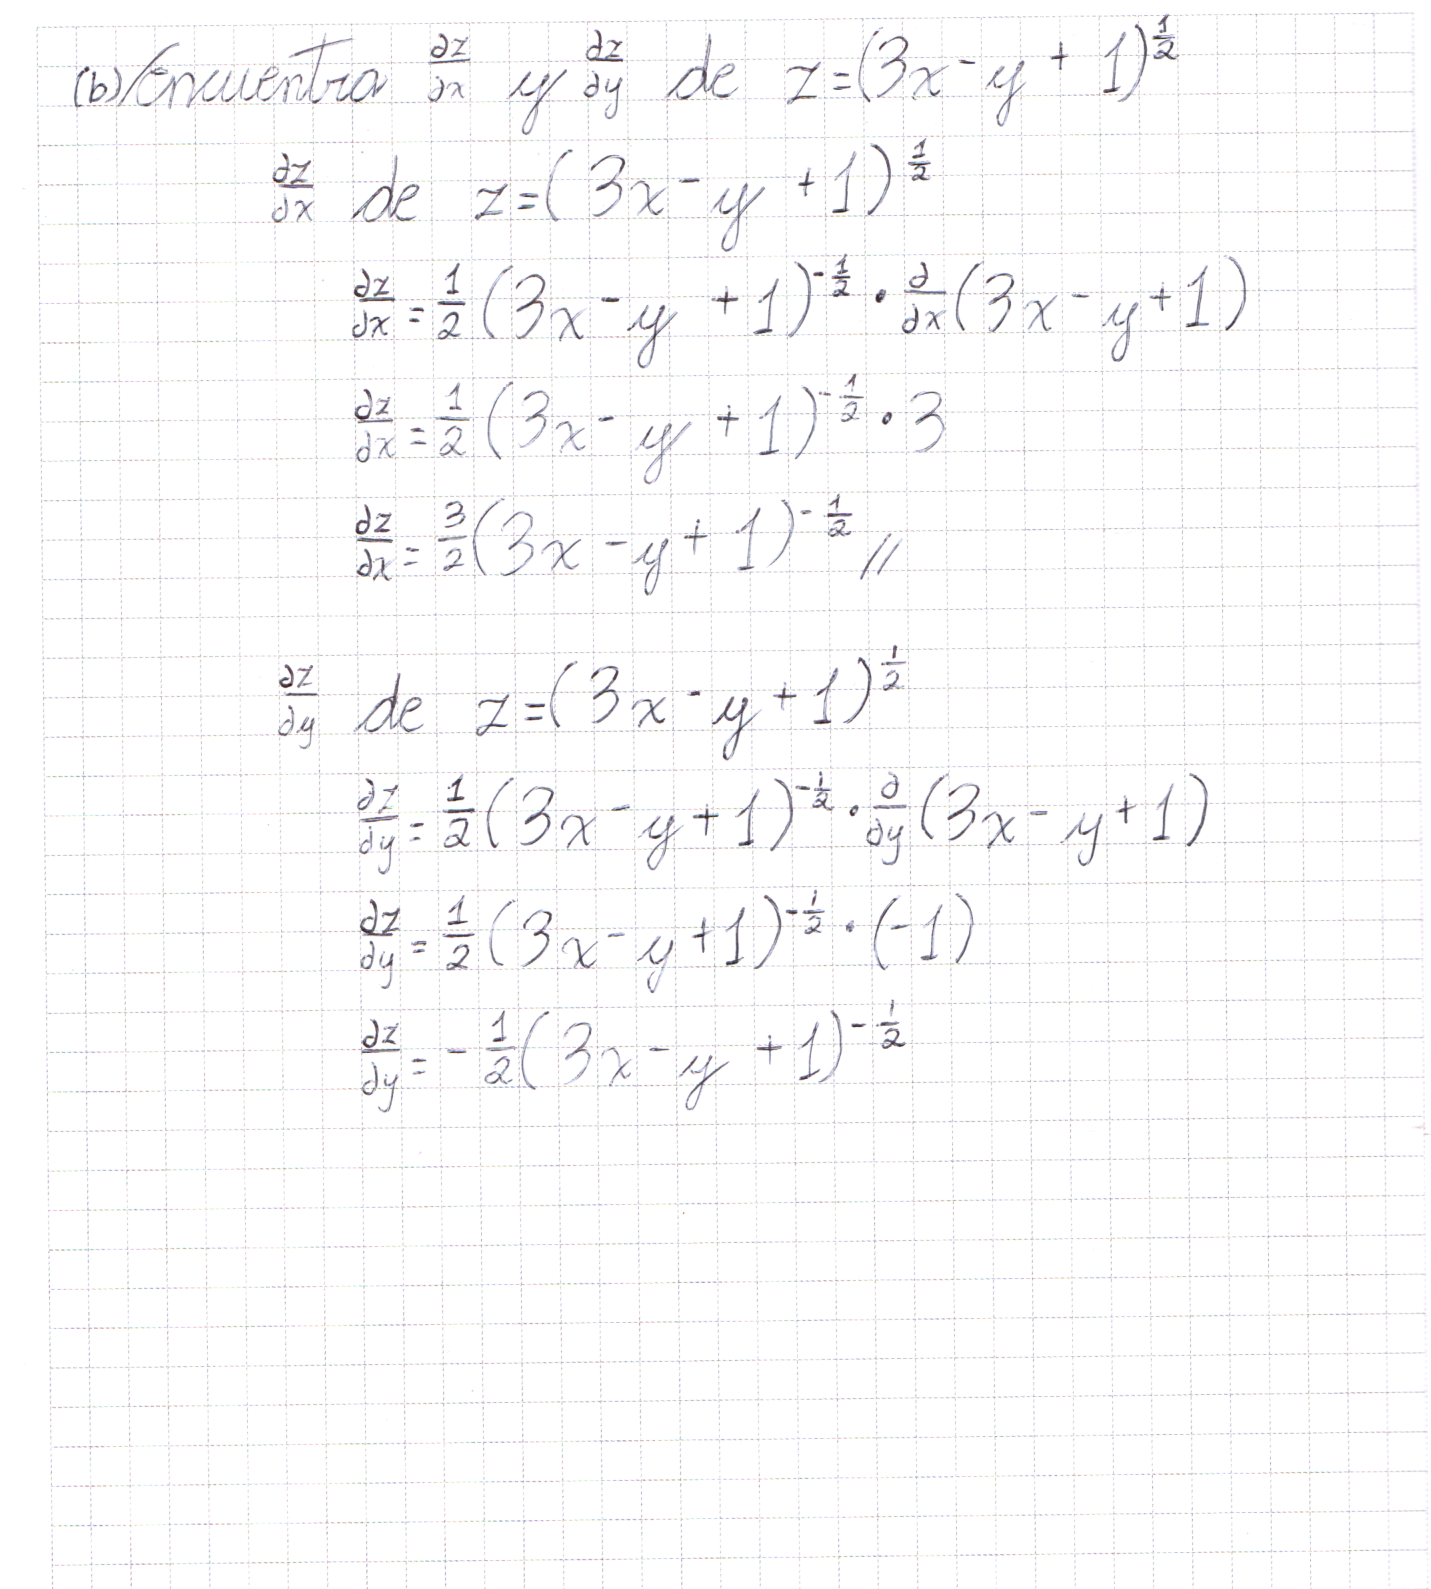
\includegraphics[width=1.1\linewidth]{/pregunta_8/8_b.png}
	\end{figure}
	\item Encuentra $\frac{\partial f}{\partial x}$ y $\frac{\partial f}{\partial y}$ de $f(x,y)=2x^2y+3xy^2$.
	\begin{figure}[H]
		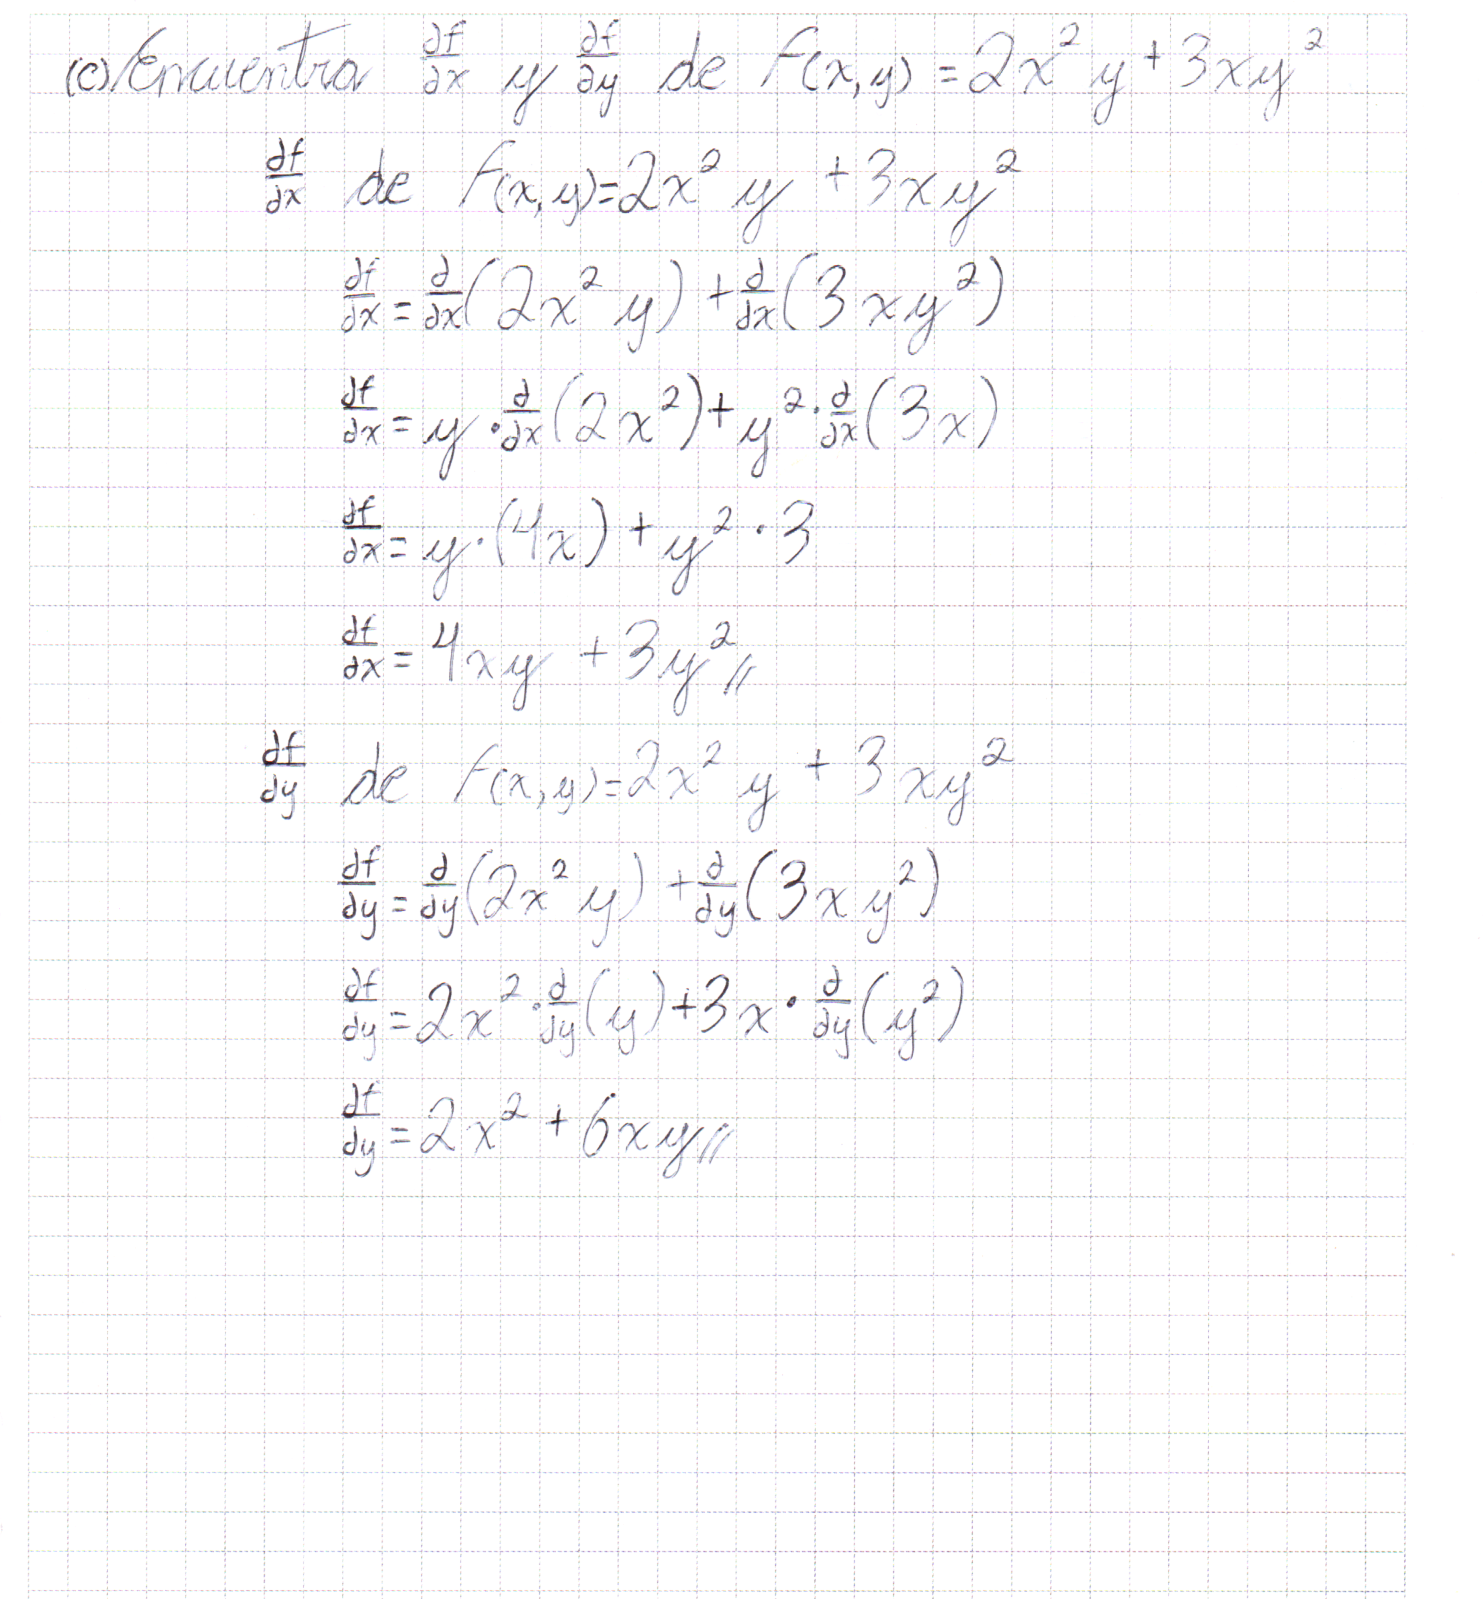
\includegraphics[width=1.1\linewidth]{/pregunta_8/8_c.png}
	\end{figure}
	\item Encuentra $\frac{\partial f}{\partial x}$ y $\frac{\partial f}{\partial y}$ de $f(x,y)=(x^2y^2+2x^3y^2)^2$.
	\begin{figure}[H]
		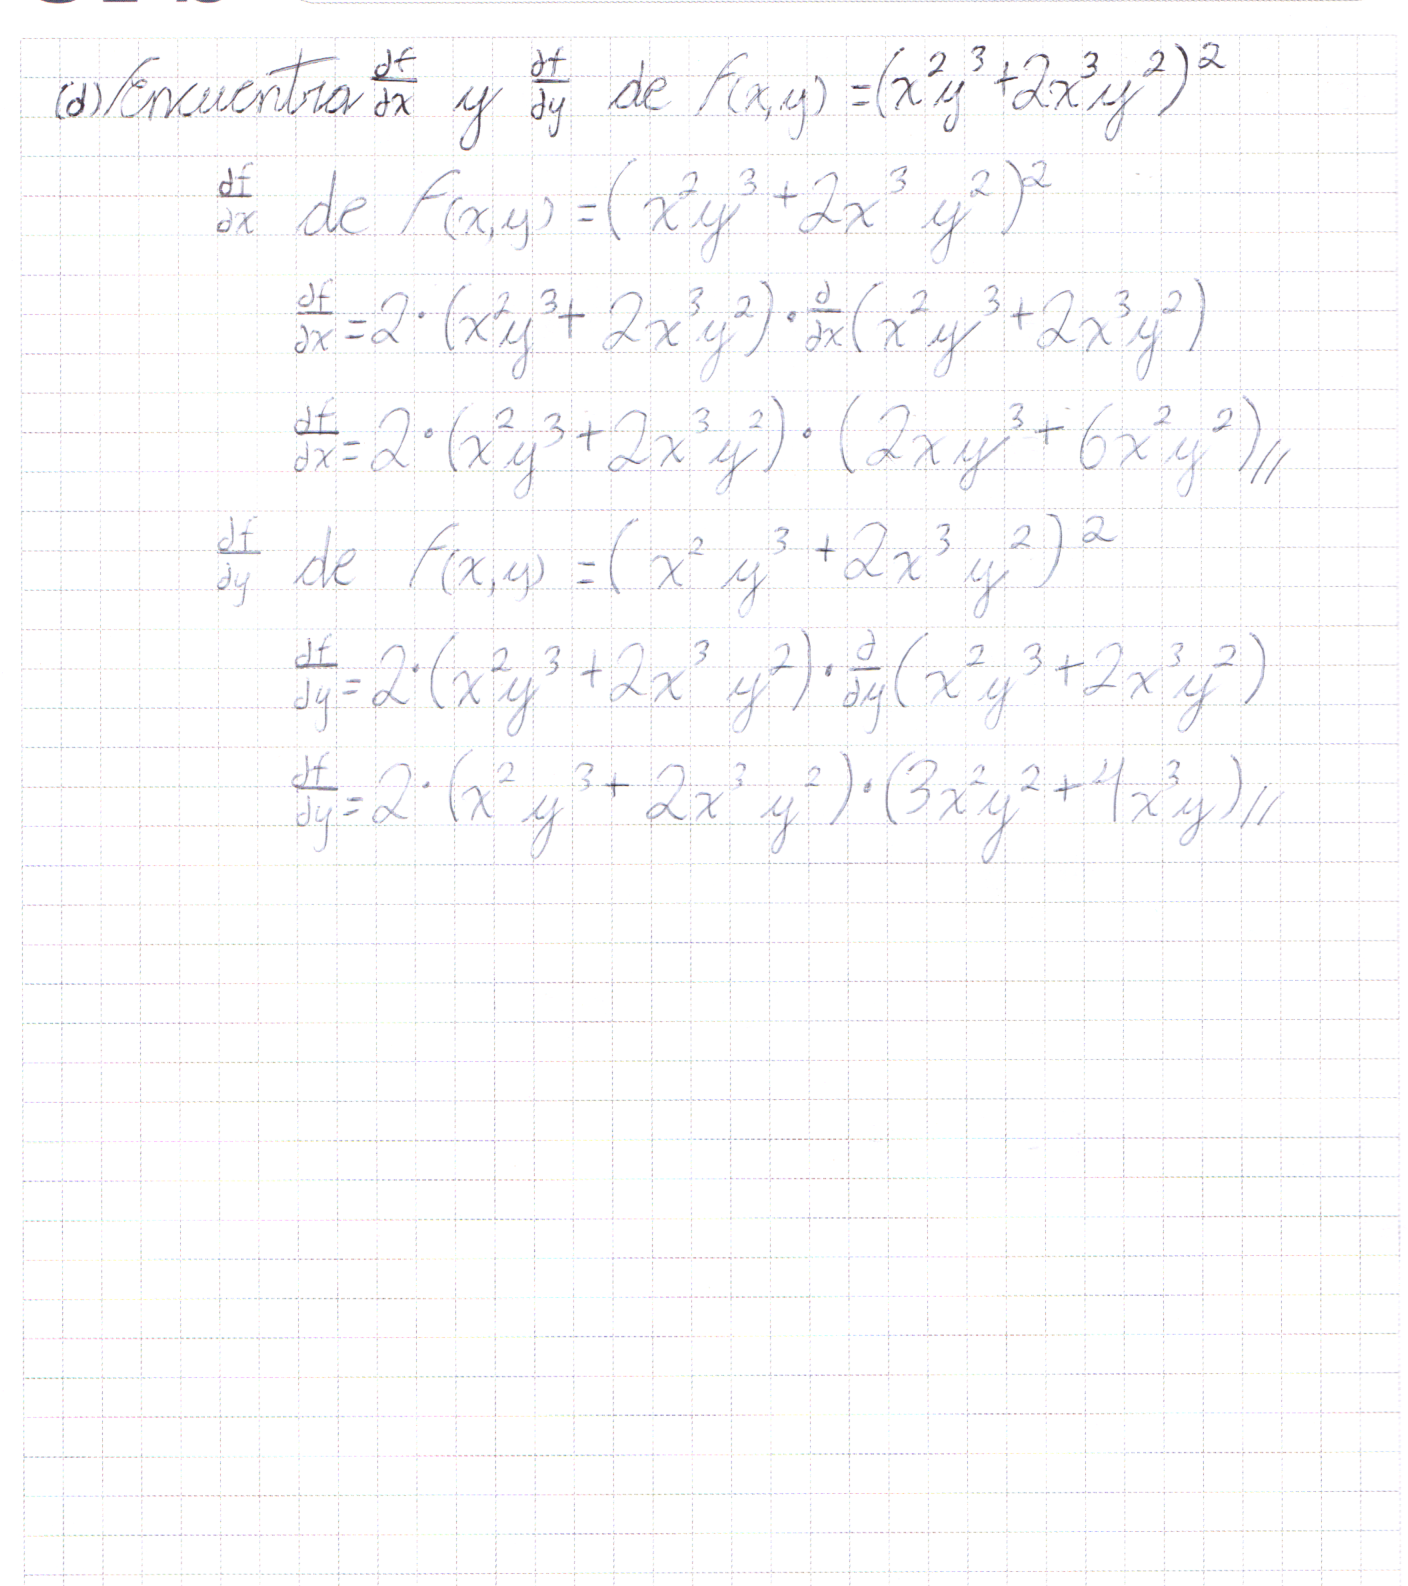
\includegraphics[width=1\linewidth]{/pregunta_8/8_d.png}
	\end{figure}
\end{enumerate}

\section*{Pregunta 9}
Utiliza la derivada de la función para encontrar el valor de $x$ que minimizan la función.

\begin{enumerate}[label=(\alph*)]
	\item Encuentra el valor de $x$ que minimiza la función $f(x)=x^2+4x+5$.
	\begin{figure}[H]
		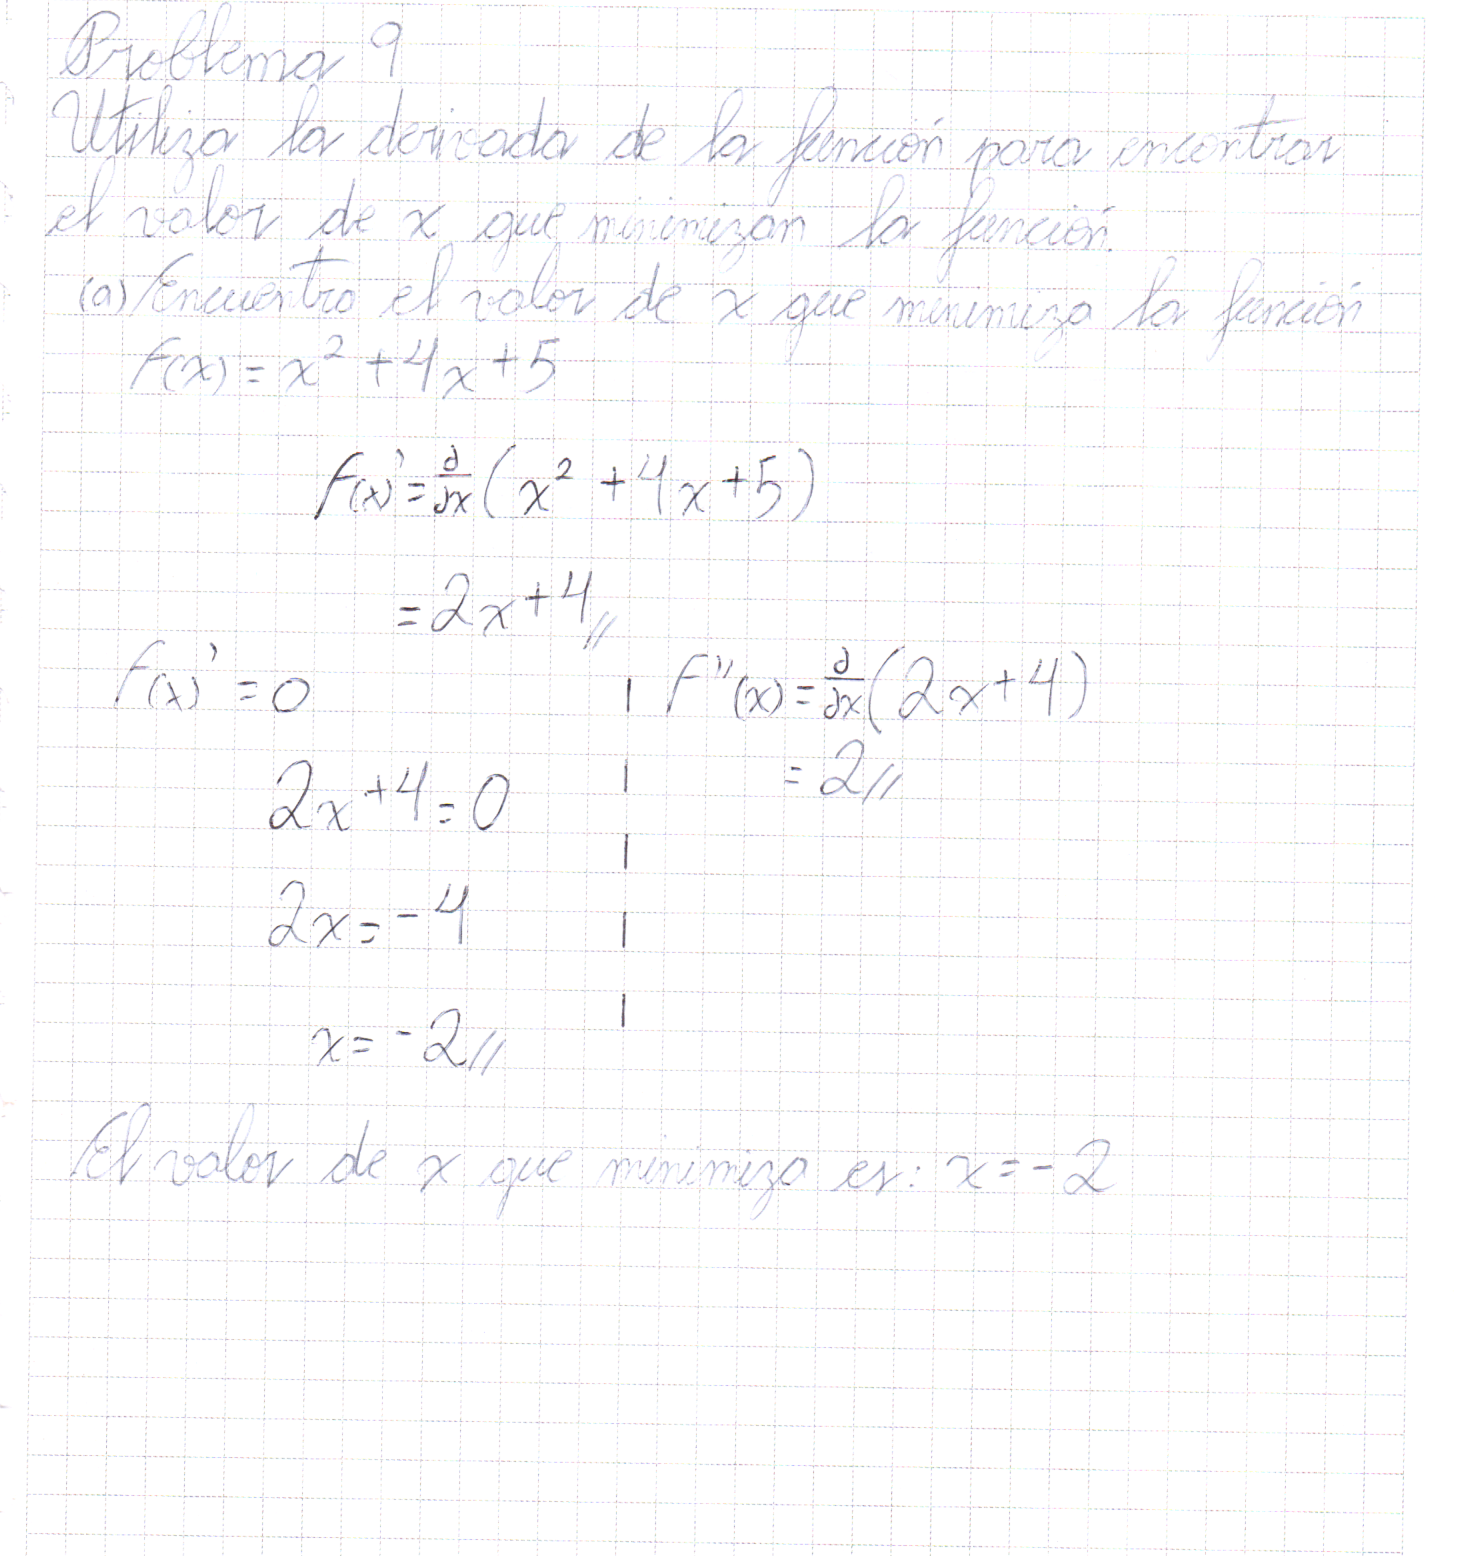
\includegraphics[width=1.06\linewidth]{/pregunta_9/9_a.png}
	\end{figure}
	\item Encuentra el valor de $x$ que minimiza la función $f(x)=(x-3)^2+7$.
	\begin{figure}[H]
		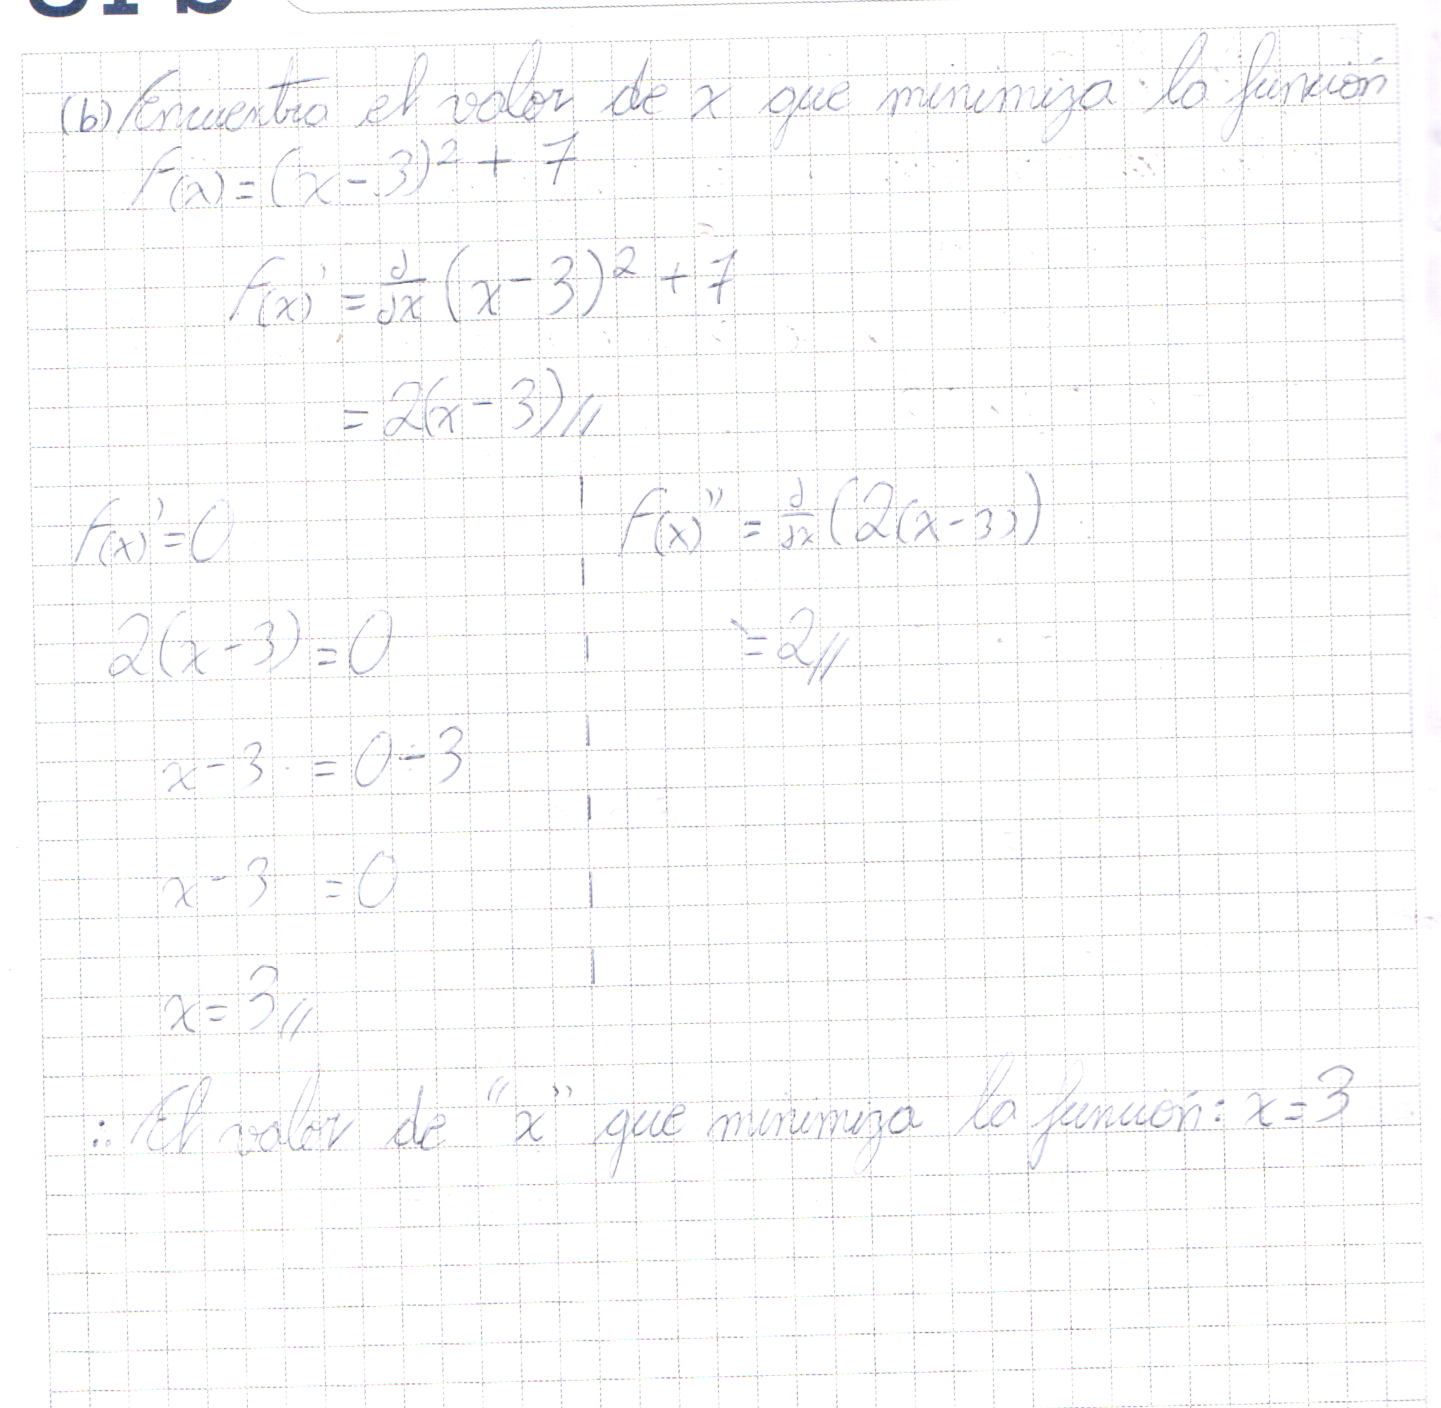
\includegraphics[width=1.15\linewidth]{/pregunta_9/9_b.png}
	\end{figure}
\end{enumerate} 

\section*{Pregunta 10}
Utiliza las derivadas parciales para encontrar los valores $x$ y $y$ que minimizan la función.

\begin{enumerate}[label=(\alph*)]
	\item Encuentra los valores de $x$ y $y$ que minimizan la función $f(x,y)=x^2+y^2$.
	\begin{figure}[H]
		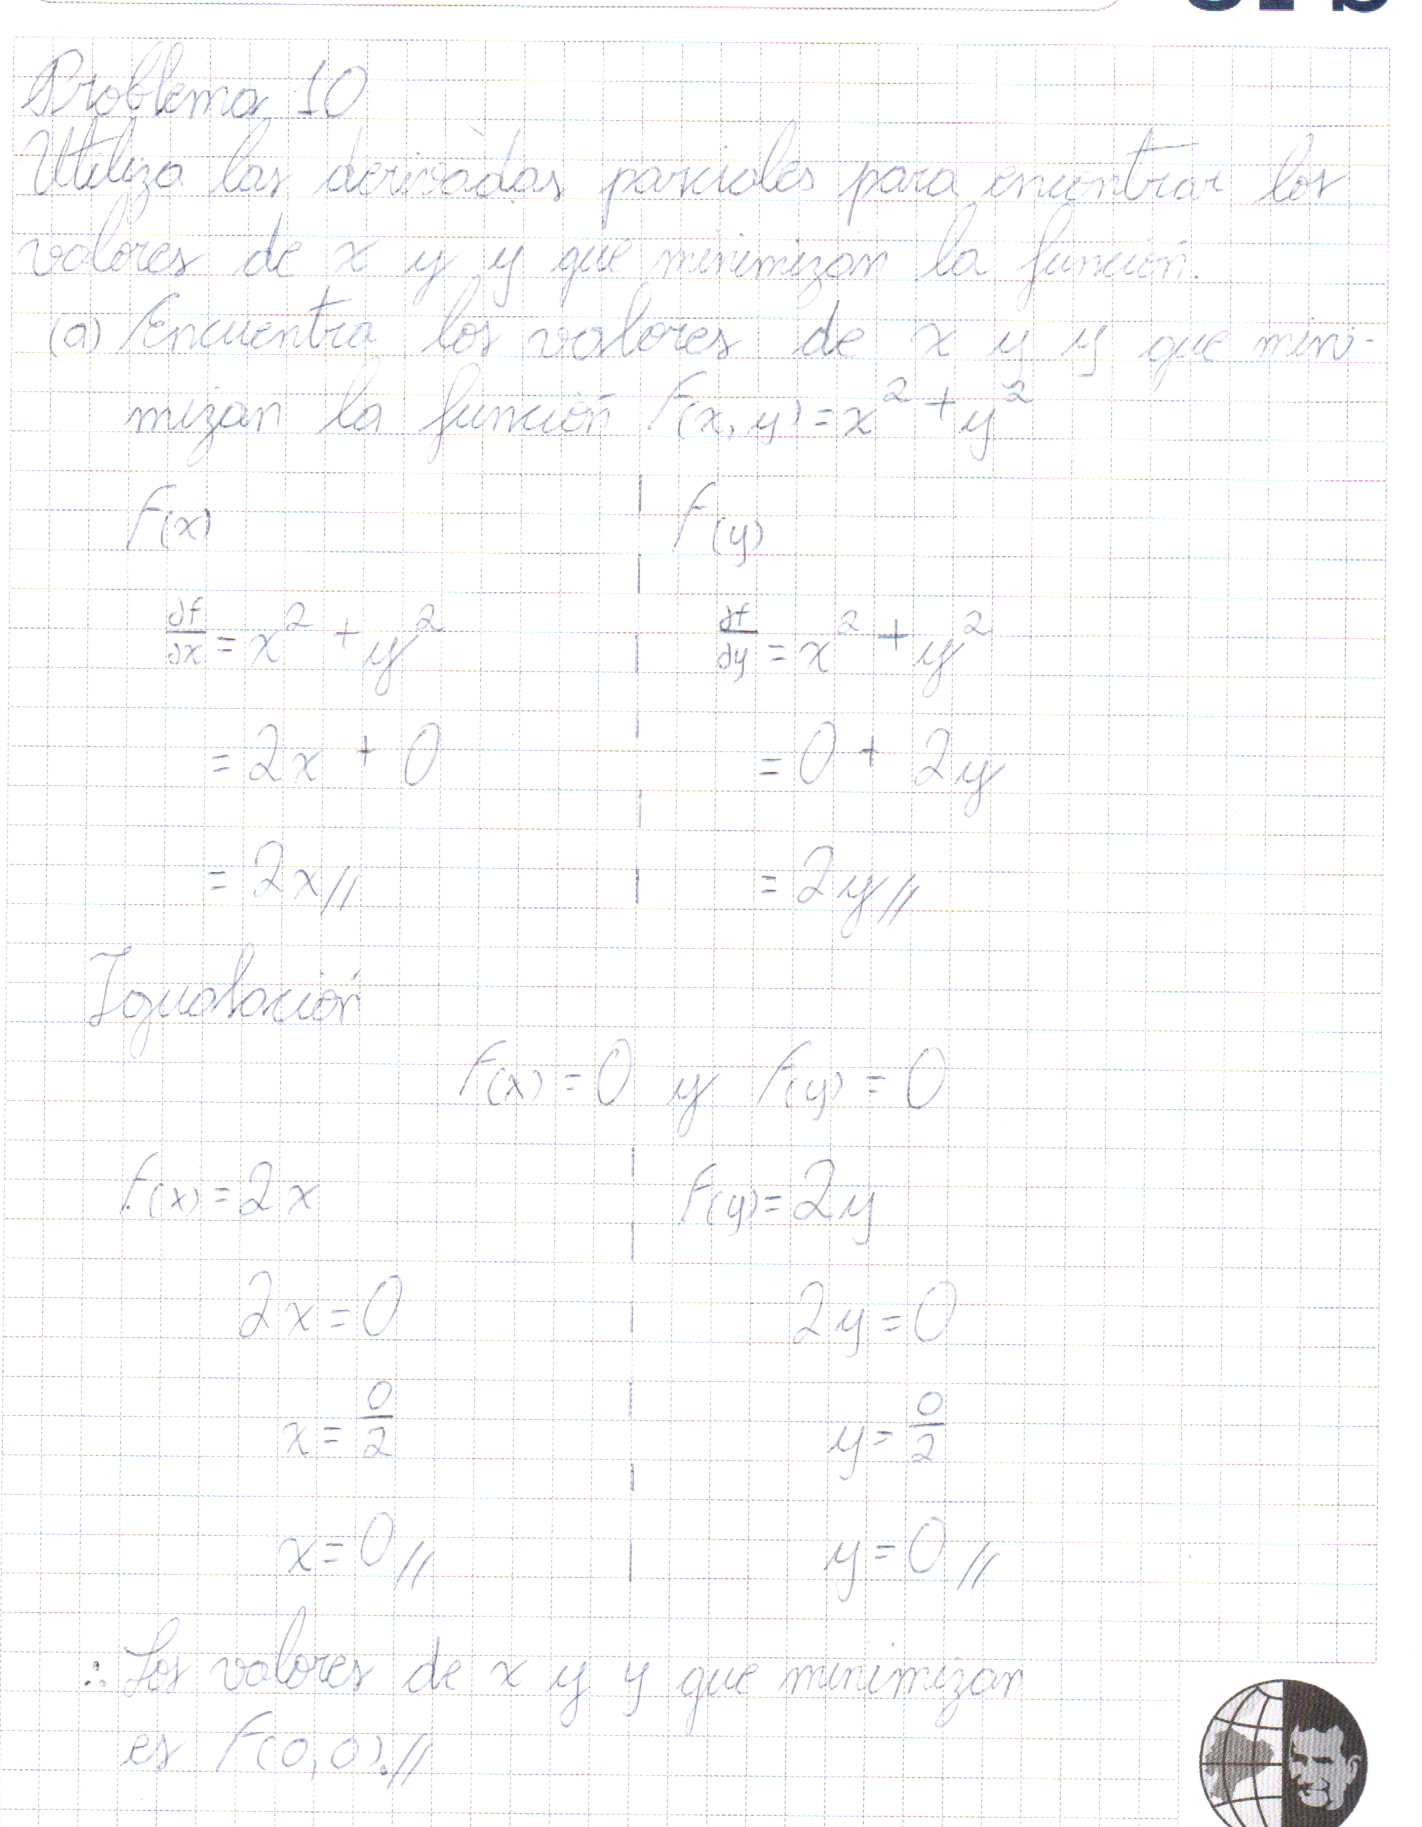
\includegraphics[width=0.86\linewidth]{/pregunta_10/10_a.png}
	\end{figure}
	\item Encuentra los valores de $x$ y $y$ que minimizan la función $f(x,y)=x^2+y^2+4x+6y+14$
	\begin{figure}[H]
		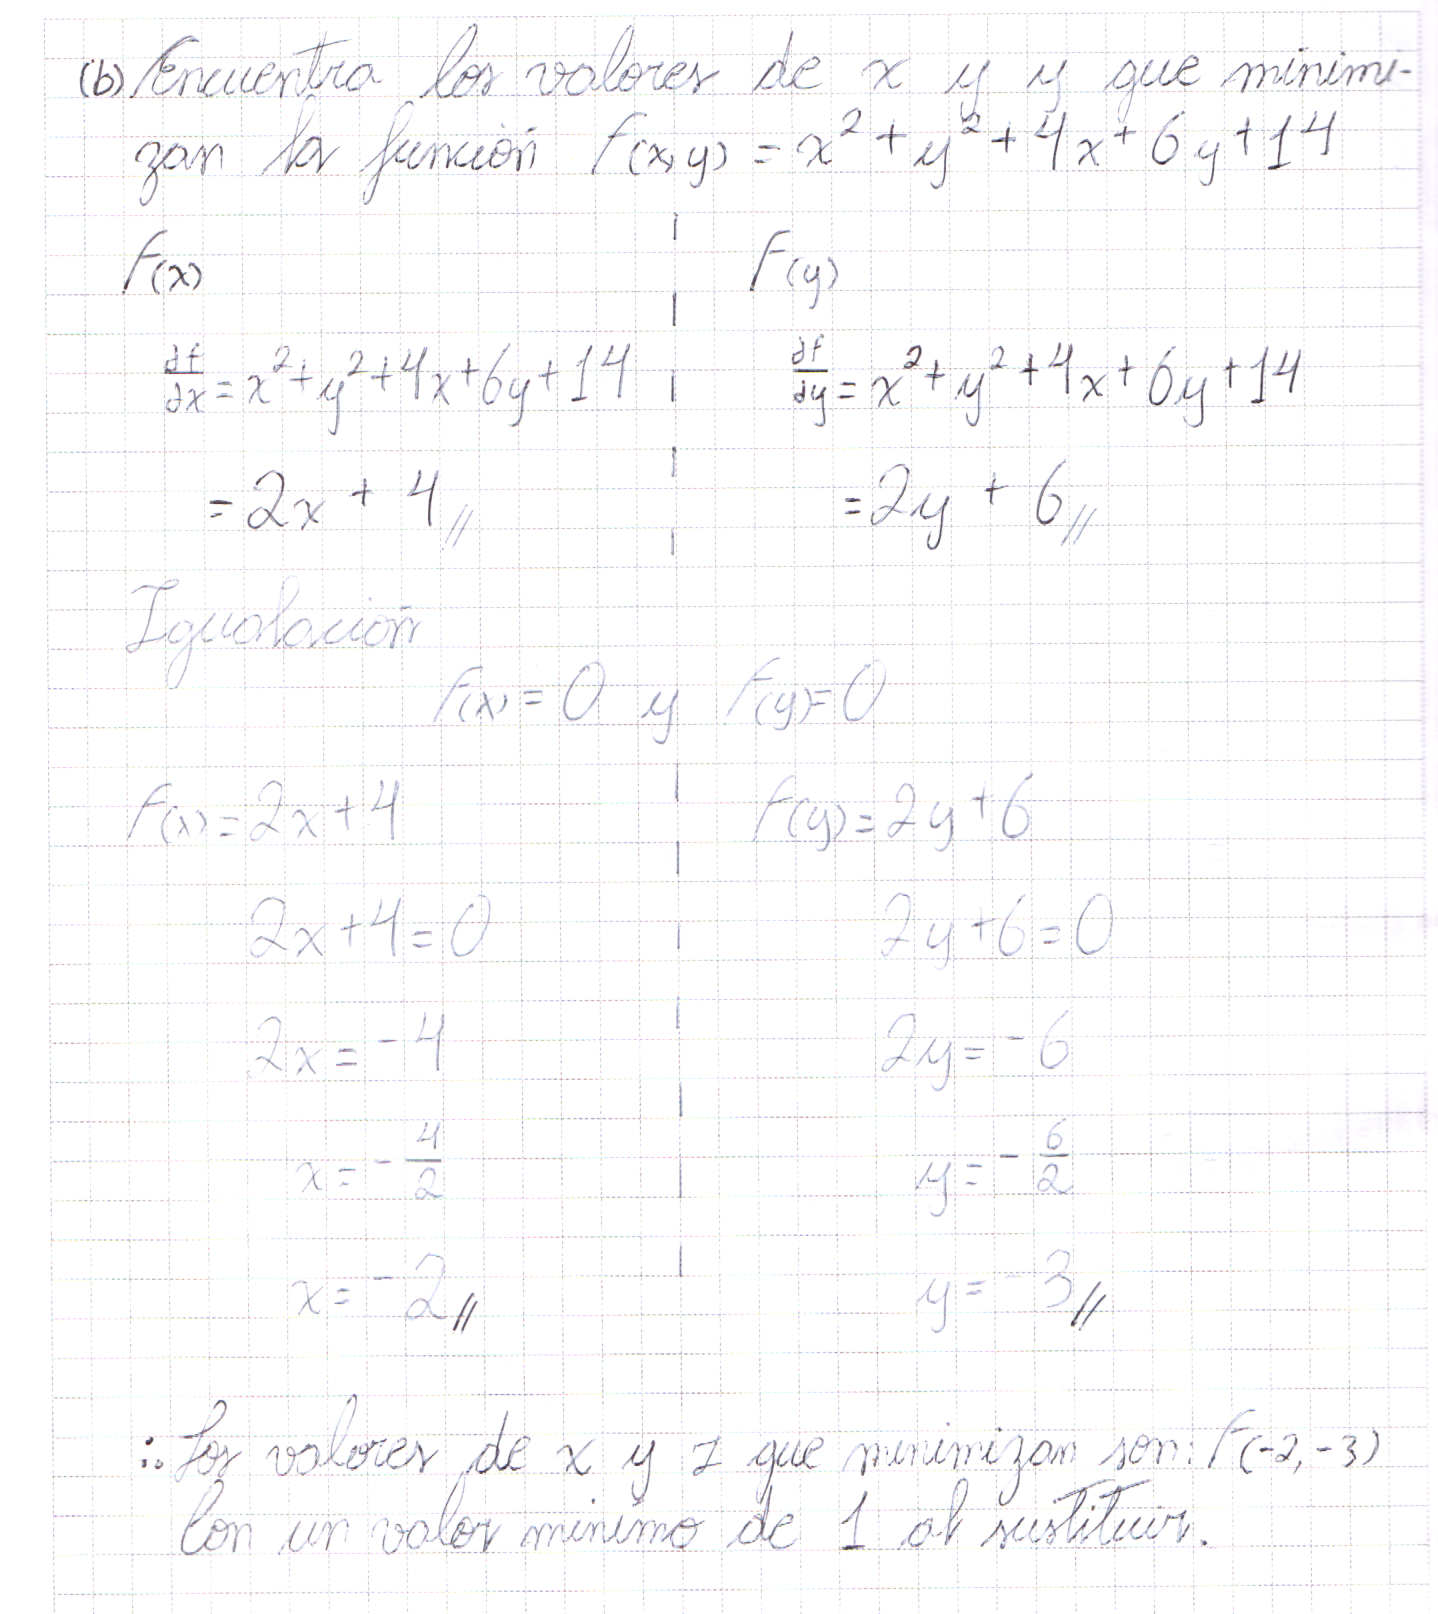
\includegraphics[width=0.98\linewidth]{/pregunta_10/10_b.png}
	\end{figure}
\end{enumerate}
\end{document}
